\documentclass[11pt]{article}
\usepackage{classTools}
\usepackage{tikz}
\usepackage{chessboard}
\usepackage{xcolor}

\begin{document}

% To include a problems set header, use the psHeader command
\psHeader{5}{Wed Oct. 23, 2024 (11:59pm)}

\textbf{Your name: } Emily

\textbf{Collaborators: } Elvin Lo

\textbf{No. of late days used on previous psets: } 0

\textbf{No. of late days used after including this pset: } 3

\medskip \noindent
\textit{Remember to mark your pages on Gradescope properly, or points will be taken off. Additionally, if your handwriting isn't particularly neat please submit written proofs, which are much easier to grade for the TFs.}

\begin{enumerate}
    \item (Solving Games) Consider playing a solo game on an $n\times n$ chessboard.  You have one piece, a chess knight, which starts in the lower-left corner, and your goal is to reach any of the other three corners in as few moves as possible.  Like a usual chess knight, in one move, you can move to any position that is two squares away in a horizontal direction and one square away in a vertical direction, or two squares away in a vertical direction and one square away in a horizontal direction.  There is a catch, however: some squares have visible landmines, so you cannot move to them (since you do not want set off an explosion). 

    \begin{enumerate}
    \item Give an algorithm that achieves the above goal in time $O(n^2)$ by reduction to either the ShortestWalks problem or the SingleSourceShortestPaths problem. The algorithm should output $\bot$ if no sequence of moves can take you to any of the other three corners when started in the lower-left corner. (Note: if reducing to SingleSourceShortestPaths, we haven't defined abstractly what it means to reduce a computational problem to a data structure problem, but you may construct and use a SingleSourceShortestPaths data structure on an appropriately constructed graph.) \\
    
    \textit{Solution. }
      Algorithm: First we construct a graph. Each tile on the board that is not a mine is a vertex on the graph. Each valid move is an edge. A valid move is as follows: From a tile/vertex that is contained in the board and is not a mine, the move is two squares in one direction and one square in a perpendicular direction. The destination tile/vertex that is moved to is contatined within the $5x5$ board and not a mine.\\
      
      Next, wish to find the shortest path to and of the other three corners from the lower left corner. If any of the corners are a mine, they are not included in the set of vertices, and therefore we return $\perp$. Otherwise, the starting vertex and ending vertex are both valid vertices, and the problem reduces to ShortestWalks. \\

      To solve ShortestWalks, we first solve SingleSourceShortestPaths, which we can solve with the class example of BFS augmented to track predecessors. \\
      
      Correctness: If our graph is correct, then our reduction, and therefore our algorithm, are both correct. Using the class notation, the graph $G$ contains all accessible vertices $V$ and can simulate any path the knight would take from the lower left tile/vertex, $s$ as a walk with our set of valid moves/edges, $E$. This is an exhaustive procedure where every path on the board can be represented on the graph $G(V,E)$. Therefore our graph is valid. Finally, we return the correct shortest path by looking at our valid paths to each of the other three corners and returning the shortest one. \\
      
      Runtime: Constructing the graph takes $O(n^2)$ time because we go create at most $n^2$ vertices by traversing the board and at most $8 * n^2 \rightarrow O(n^2)$ edges since each tile/vertex on the board can have up to 8 valid moves/edges. Therefore when we run the predecessor augmented BFS, the runtime is $O(n^2)$ time. We do this 3 times for each of the three other corners. Therefore our runtime is donminated by $\boxed{O(n^2)}$. \\

    \item Carry out your algorithm on the $5\times 5$ board shown below, listing both the frontier vertices and the predecessor relationships at each stage of BFS (the red square symbols are landmines).
    
    \begin{figure} [H]
    \centering
    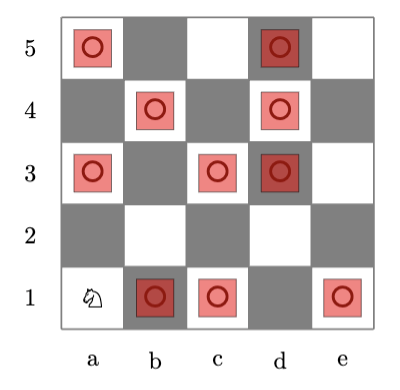
\includegraphics[width=0.4\linewidth]{chessboard.png}
    % \begin{tikzpicture}
    %     \definecolor{white}{rgb}{1,1,1}
    %     \definecolor{black}{rgb}{0.5,0.5,0.5}
    %     \definecolor{darkred}{rgb}{0.6, 0, 0}

    %     \def\landmines{(2.5,1.5), (1.5,5.5), (5.5,1.5), (1.5,3.5), (3.5,1.5),(3.5,3.5),(4.5,4.5),(4.5,5.5),(2.5,4.5), (4.5,3.5)}
        
    %     % Loop to create the 5x5 grid
    %     \foreach \x in {1,...,5} {
    %         \foreach \y in {1,...,5} {
    %             % Alternate black and white squares
    %             \pgfmathparse{mod(\x+\y,2)}
    %             \ifnum\pgfmathresult=0
    %                 \fill[white] (\x, \y) rectangle ++(1,1);
    %             \else
    %                 \fill[black] (\x, \y) rectangle ++(1,1);
    %             \fi
    %         }
    %     }
    
    %     % X-axis labels
    %     \foreach \x/\letter in {1/a, 2/b, 3/c, 4/d, 5/e} {
    %         \node at (\x+0.5, 0.5) {\letter}; 
    %     }
    
    %     % Y-axis labels
    %     \foreach \y in {1, 2, 3, 4, 5} {
    %         \node at (0.5, \y+0.5) {\y};  
    %     }
    
    %     % Knight symbol
    %     \node at (1.5, 1.5) {\knight};

    %     %Adding landmines
    %     \foreach \position in \landmines {
    %         \draw[fill=red, opacity=0.5] \position ++(-0.3,-0.3) rectangle ++(0.6,0.6); 
    %         \node at \position {\textcolor{darkred}{\Huge$\circ$}};  
    %     }
    
    %     % Grid lines
    %     \draw[step=1cm,black,thick] (1,1) grid (6,6);
        
    % \end{tikzpicture}
    \end{figure}
    \textit{Solution. }
    \begin{center}
      \begin{tabular}{|c|c|c|}
          \hline
          \textbf{Distance from (a,1)} & \textbf{Predecessor} & \textbf{Frontier} \\
          \hline
          0 & - & (a,1) \\
          \hline
          1 & (a,1) & (b,3), (c,2) \\
          \hline
          2 & (b,3) & (c,5), (d,2) \\
          2 & (c,2) & (e,3) \\
          \hline
          3 & (c,5) & (a,4), (e,4) \\
          3 & (d,2) & (c,4) \\
          3 & (e,3) & (d,1) \\
          \hline
          4 & (a,4) & (b,2) \\
          4 & (e,4) &   \\
          4 & (c,4) & (e,5) \\
          \hline
      \end{tabular}
    \end{center}
    Return $(a, 1) \rightarrow(c, 2) \rightarrow(e, 3) \rightarrow$ $(c, 4) \rightarrow(e, 5)$.
    \end{enumerate}


 \item (Maximal Independent Sets) Let $G=(V,E)$ be a graph.  A set $S\subseteq V$ is a {\em maximal} independent set if we cannot add any vertices to $S$ while it remains an independent set.  That is, for every vertex $v\in V\setminus S$, $S\cup\{v\}$ is not an independent set.
    \begin{enumerate}
        \item Show that given a graph $G$, a maximal independent set can be found in time $O(n+m)$.  Note that this is in sharp contrast to {\em maximum-size} independent sets, for which we do not know any subexponential-time algorithms. (Hint: be greedy.) \\
        
        \textit{Solution. }
        We will write out a greedy search algorithm to fin a maximal independent set:
        \begin{enumerate}
          \item Initialize $S = \emptyset$ to be the maximal independent set, $T = V$ to be the set of vertices to be visited.
          \item Pick some $v \in T$. Then remove $v$ and all of its neighbors from $T$. Continue this process until $T$ is empty.
          \item Correctness: By construction, $S$ is an independent set. $S$ is maximal since it considered all of $V$. No $v \in V$ that is not already in $S$ can be added to $S$ and retain set independence, since all other $v$ not in $S$ are a neighbor some element of $S$.
          \item Runtime: Let $n$ be the number of vertices and $m$ be the number of edges. Initializing $S$ and $T$ takes $O(1)$ and $O(n)$ time. Each $n$ vertices are processed once, which takes $O(n)$ time. For each vertex, we check its edges. This takes time proportional to the degree of the vertex. The total sum of the degrees of all vertices in the graph is $2 m \rightarrow O(m)$. The overall runtime is therefore $O(n+m)$.
        \end{enumerate}
        
        \item Show that if $G$ is 3-colorable, then it has a 3-coloring $f$ in which the set of vertices of color 2 (i.e. $f^{-1}(2)$) is a maximal independent set. \\

        \textit{Solution. } If a graph $G$ is 3-colorable, its vertices can be colored using three colors which means that for colors 1, 2, and 3, and coloring $f$m $f^{-1}(1), f^{-1}(2), f^{-1}(3)$ are independent sets. Now we will show that if this is the case, we can construct $f^{-1}(2)$ as a maxiamal independent set.

        To start, assume $f^{-1}(2)$ is not maximal. But then we can add some $v$ that is either color 1 or 3 and is independent of $f^{-1}(2)$. Then we can add $v$ to $f^{-1}(2)$ without violating the independence property, since $v$ is independent of $f^{-1}(2)$. Then we repeat this until there are no more such $v$, in which case $f^{-1}(2)$ is maximal independent set.

        This is correct because by construction, $f^{-1}(2)$ is a maximal independent set. Also, the remaining $f^{-1}(1), f^{-1}(3)$ are independent sets because they are subsets of the original independent sets. Thus, $f$ is a valid coloring, so we have shown that if $G$ is 3 -colorable, then there exists a 3 -coloring $f$ such that $f^{-1}(2)$ is a maximal independent set. \\

        \item It is known that every graph $G$ has at most $3^{n/3}$ maximal independent sets, and there is an algorithm (the Bron-Kerbosch algorithm) that enumerates all of the maximal independent sets in time $O(3^{n/3}).$  Use this fact to conclude that 3-coloring can be solved in time $O((n+m)\cdot 3^{n/3}) = O(1.44^n),$ improving the runtime of $O(1.89^n)$ from SRE4.\\
        
        To find a valid 3-coloring, we can enumerate all the possible maximal independent sets $S$ using Bron-Kerbosch. Then for each $S$, we may create a new graph $G^{\prime}$ which is $G$ with all the vertices and associated edges in $S$ removed. Finally, wecheck that $G^{\prime}$ is 2-colorable using BFSColoring. If the $G^{\prime}$ is 2-colorable, then we return the coloring of $G$ with  $S$ is color 2 and $G^{\prime}$ maps to colors 1 and 3 .

        This coloring is correct because $S$ is an independent set, and BFSColoring returns a correct 2-coloring. From part b, we can then show the runtime. First we generate all maximal independent sets $S$ in time $O(3^{n / 3})$. For each $S$, create $G^{\prime}$, which takes $O(n+m)$ time. We also do BFSColoring on $G^{\prime}$, which has $O(n)$ vertices and $O(m)$ edges. Therefore BFSColoring takes $O(n+m)$ time. Therefore the final runtime is $O\left((n+m) \cdot 3^{n / 3}\right)$.
    \end{enumerate}
 
\newpage
 \item (Exponential-Time Coloring) 
  In the \href{https://github.com/Harvard-CS-120/cs120/tree/main/fall2022/psets}{Github repository} for PS5, we have given you basic data structures for graphs (in adjacency list representation) and colorings, an implementation of the Exhaustive-Search $k$-Coloring algorithm, 
  an implementation of the Bron-Kerbosch algorithm, and a variety of test cases (graphs) for coloring algorithms. 

  \begin{enumerate}
      \item Implement the $O(n+m)$-time algorithm for 2-coloring that we covered in class in the function \texttt{bfs\_2\_coloring}, verifying its correctness by running \texttt{python3 -m ps5\_tests 2}.
        Your implementation of BFS should follow the presentation and notation that we used in class (with the loop over distance $d$ and the sets $F$ and $S$), which may be different than presentation of BFS in other sources (online or in the optional textbooks). 
        
      \item Implement the $O((n+m)\cdot 3^{n/3})$-time algorithm for 3-coloring (MaximalIS + BFS) from Problem 2 above in the function \texttt{iset\_bfs\_3\_coloring}, also verifying its correctness by running \texttt{python3 -m ps5\_tests 3}. \label{part:TbT}
    
    \item Compare the efficiency of Exhaustive-Search 3-coloring and the $O((n+m)\cdot 3^{n/3})$-time algorithm. Specifically, identify and write down the largest instance size $n$ each algorithm is able to solve (within a time limit you specify, e.g. 1 second) and the smallest instance size $n$ each algorithm is unable to solve (again within that same time limit). 
    
    In addition to these numeric values, please provide a brief explanation of why these results make sense, based on your knowledge of both the algorithms' runtime and how each algorithm goes about finding a coloring. For this part, there is no need to go through every combination of parameters; feel free to give just the largest and smallest instances each algorithm can solve and speak generally as to why one algorithm performs better than the other. More instructions can be found in \texttt{ps5\_experiments}. \\

    \textit{Solution. }
    The time limit specified was 1 second. The results of running the experiments showed that the largest instance size \( n \) that \textbf{Exhaustive-Search 3-Coloring} was able to solve is \( n = 20 \), and the smallest instance size \( n \) that it was unable to solve is \( n = 36 \). The largest instance size \( n \) that \textbf{ISET BFS Coloring} was able to solve is \( n = 72 \), and the smallest instance size \( n \) that it was unable to solve is \( n = 72 \) with increased edge density.

    This demonstrates that ISET BFS Coloring performs significantly better in handling larger graphs within the 1-second time constraint compared to Exhaustive-Search.

    This may make sense because the Exhaustive Search 3-coloring algorithm checks every possible way to assign one of three colors to each of the \( n \) vertices. This leads to \( 3^n \) possible configurations, and for each one, it verifies all \( m \) edges to ensure no two adjacent vertices share the same color. This approach grows exponentially with \( n \), quickly becoming impractical, even for small $n$.

    The Maximal Independent Sets + Breadth-First Search (BFS) method takes a different approach by breaking the problem down into smaller tasks. First, it finds \textit{maximal independent sets}—groups of vertices that are not adjacent to each other and can’t be expanded without losing that property. It colors each maximal independent set with a single color. Then, it checks if the rest of the graph can be colored with just two colors, a simpler task than 3-coloring. This is done using BFS, which is efficient.

    Instead of considering every possible coloring configuration (which grows as \( 3^n \)), the Maximal Independent Sets + BFS approach only considers configurations related to independent sets. This reduces the complexity from \( 3^n \) to about \( 3^{n/3} \), a substantial improvement. While the BFS verification step takes \( O(n + m) \) time, this polynomial factor is manageable compared to the exponential savings from focusing on independent sets.

    Overall, the Maximal Independent Sets + BFS approach is much more efficient and can handle larger graphs. While Exhaustive Search fails when \( n \) reaches around 30, the Maximal Independent Sets + BFS method can handle graphs with up to 72 vertices before it times out. In short, the Maximal Independent Sets + BFS method is far more efficient because it focuses only on relevant subsets of vertices (independent sets) and uses a fast BFS-based 2-coloring check. This makes it feasible to solve much larger graphs than the Exhaustive Search method, which quickly becomes impractical as the graph size grows.
    
  \end{enumerate}
  
  

\item (Reflection): Take one homework problem you have worked on this semester that you struggled to understand and solve, and explain how the struggle itself was valuable.  In the context of this question, describe the struggle and how you overcame the struggle. You might also discuss whether struggling built aspects of character in you (e.g. endurance, self-confidence, competence to solve new problems) and how these virtues might benefit you in later ventures. 

 \textit{Note: As with the previous psets, you may include your answer in your PDF submission, but the answer should ultimately go into a separate Gradescope submission form.}

 \textit{Quick note on grading: Good responses are usually about a paragraph, with something like 7 or 8 sentences. Most importantly, please make sure your answer is specific to this class and your experiences in it. If your answer could have been edited lightly to apply to another class at Harvard, points will be taken off.}

\item Once you're done with this problem set, please fill out \href{https://forms.gle/pR1Mt4PmMhUfuW1G6}{this survey} so that we can gather students' thoughts on the problem set, and the class in general. It's not required, but we really appreciate all responses!
\end{enumerate}

\end{document}